\cleardoublepage
\phantomsection
\chapter{Quick Start}

\begin{quote}
\textit{Software engineering is what happens to programming when you add time,
and other programmers.} -- Russ Cox
\end{quote}

This chapter walks through a few basic topics in Go. You should be able to write
simple programs using Go after reading and practicing the examples given in this
chapter. The next 3 sections revisit the hello world program introduced in the
last chapter. Later we will move on to a few basic topics in Go. We will learn
about data types, variables, comments, For loops, range clauses, If, functions,
operators, slices, and maps.

\section{Hello World!}

Here is the hello world program introduced in the previous chapter.
You can type the below code to your favorite text editor and save it
as \texttt{hello.go}.  This program will print a
message, \texttt{Hello, World!} into your console/terminal.

\lstinputlisting[caption=Hello World]{code/quickstart/hello.go}

You can open your command line program and run the above program like
this:

\begin{lstlisting}[numbers=none]
$ go run hello.go
Hello, World!
\end{lstlisting}

What you wrote in the \texttt{hello.go} is a structured document.  The
characters, words, spaces, line breaks and the punctuation characters
used all are important.  In fact, we followed the "syntax" of Go
language.  According to Wikipedia, the syntax of a computer language
is the set of rules that defines the combinations of symbols that are
considered to be a correctly structured document or fragment in that
language.

The \texttt{go run} command is easy to use when developing programs.
However, when you want to use this program in production environment,
it is better to create executable binaries.  The next section briefly
explain the process of building executable binaries and running it.

\section{Building and Running Programs}

You can use the \texttt{go build} command to compile the source and
create executable binary programs.  Later this executable can run
directly or copied to other similar systems and run.

To compile (build) the hello world program, you can use this command:

\begin{lstlisting}[numbers=none]
$ go build hello.go
\end{lstlisting}

This command produce an an executable file named \texttt{hello} in the
current directory where you run the \texttt{build} command.  And you
can run this program in a GNU/Linux system as given below.
The \texttt{./} in the beginning of the command ensure that you are
running the \texttt{hello} program located in the current directory:

\begin{lstlisting}[numbers=none]
$ ./hello
Hello, World!
\end{lstlisting}

In Windows, the executable file name ends with \texttt{.exe}.  This is
how you can run the executable in Windows:

\begin{lstlisting}[numbers=none]
C:\> hello.exe
Hello, World!
\end{lstlisting}

The \texttt{go build} command produce a binary file native to the
operating system and the architecture of the CPU (i386, x86\_64, arm
etc.)

\section{The Example Explained}

The first line is a clause defining the name of the package to which
the file belongs.  In the above hello world program,
the \texttt{hello.go} file belongs to the the \texttt{main} package
because of this clause at the beginning of the file:

\begin{lstlisting}[numbers=none]
package main
\end{lstlisting}

A package is a collection of Go source files.  Package sources can be
spread across multiple source files in a directory.  If you want to
produce an executable from your program, the name of package should be
named as \texttt{main}.  Always use lowercase letters for the package
names.

The second line has kept as blank for readability.  The 3rd line is an
\texttt{import} declaration.  The \texttt{import} declaration enable accessing
external packages from the current package.  In the above example,
\texttt{fmt} package is imported like this.

\begin{lstlisting}[numbers=none]
import "fmt"
\end{lstlisting}

If a package is imported, it must be used somewhere in the source
files.  Otherwise, the compiler will produce an error.  As you can see
above, the import declaration starts with a word \texttt{import}
followed by the name of the package in double quotes.  If multiple
packages need be imported, you can group the imports into a
parenthesis (factored import) to reduce typing.  Here is an example
for factored import:

\begin{lstlisting}[numbers=none]
import (
    "fmt"
    "math"
)
\end{lstlisting}

The name of the package for the built-in packages will be the name given within
quotes of the import statement. If the import string is a path separated by
slash, then name of the package will be the last part of the string. For
example, "net/http" package name is \texttt{http}. For other third party vendor
packages, the name should be verified within the source code.

Names within the imported package can be referred using a dot operator as you
can see above: \texttt{fmt.Println}. A name is considered as exported if it
begins with a capital letter. For example, the name
\texttt{Area} is an exported name, but \texttt{area} is not exported.

The \url{https://go.dev/play} site can be used to share Go source code publicly.
You can also run the programs in the playground.

Again we have added one blank line after the import statement for readability.
The fifth line starts with a function definition. In this case, this is a
special function named \texttt{main}. A function is a collection of instructions
or more specifically statements. A function definition starts with \texttt{func}
keyword followed by function name then arguments (parameters) for the function
within parenthesis and finally statements within curly brackets.
The \texttt{main} function is a special function which doesn't accept any
arguments. The starting curly bracket should be in the same line where function
definition started and statements should start in the next line. There should be
only one \texttt{main} function for an executable program.

Inside the main function, we are calling the \texttt{Println} function available
inside the \texttt{fmt} package.

\begin{lstlisting}[numbers=none]
fmt.Println("Hello, World!")
\end{lstlisting}

The above function call is a complete statement in Go.
The \texttt{Println} function print the string into standard output of
the terminal/console and also add a new line at the end of the string.

\section{Organizing Code}

As mentioned above, a package is a collection of Go source files. Package
sources can be spread across multiple source files in a directory. For a given
package, all the variables, functions, types, and constants defined in one
source file can be directly referrenced from other sources files.

A Git repository normally contain one module, located at the root, however it is
possible to add more than one, if necessary. A Go module is a collection of Go
packages that are released together.

To understand the code organization, you also need to understand about Go
module. A file named \textit{go.mod} declares the module path: the import path
prefix for all packages within the module. The module contains the packages in
the directory containing its go.mod file as well as subdirectories of that
directory, up to the next subdirectory containing another go.mod file (if any).

Note that you don't need to publish your code to a remote repository before you
can build it. A module can be defined locally without belonging to a repository.
However, it's a good habit to organize your code as if you will publish it
someday.

Each module's path not only serves as an import path prefix for its packages,
but also indicates where the go command should look to download it. For example,
in order to download the module golang.org/x/tools, the go command would consult
the repository indicated by https://golang.org/x/tools (described more here).

An import path is a string used to import a package. A package's import path is
its module path joined with its subdirectory within the module. For example, the
module github.com/google/go-cmp contains a package in the directory cmp/. That
package's import path is github.com/google/go-cmp/cmp. Packages in the standard
library do not have a module path prefix.

\section{Basics}

\subsection{Data Types}

Data\index{type!built-in} is unorganized facts that requires
processing.  In programming, the data is processed and organized to be
useful.  Data type provides a classification for the data.  Date type
is often simply called as
\textit{type}.  Data type is one of the fundamental concept in any
programming language.  In most of the places in this book, we will say
data as "value".  More advanced data type is often called data
structures.

Consider an example, you want to work with names of toys in your
programs.  So, the values of the "names of toys" is the data.  The
data type that you can use to represent this data is called "string".
If you are literally writing a string in Go, you can use a double
quote around the names like this:

\begin{lstlisting}[numbers=none]
"Sheriff Woody"
"Buzz Lightyear"
"Jessie"
\end{lstlisting}

In the hello world example, we used the string "Hello, World!"
literally.  Representation of a string value within source code is
called string literal.

Consider a related example, you want to mark whether the toys are male
or not.  This type of data is called Boolean data.  So, if the toy is
male, the value will be \texttt{true} otherwise \texttt{false} as
given below:

\begin{lstlisting}[numbers=none]
{"Sheriff Woody",  true}
{"Buzz Lightyear", true}
{"Jessie",        false}
\end{lstlisting}

Apart from \textit{string}, and \textit{bool}, Go has some other data
types like \textit{int}, \textit{byte}, \textit{float64} etc.

\subsection{Variables}

Let's go back to the hello world example, if you want to print the
hello world message three times.  You will be required to write that
sentence three times as given below.

\lstinputlisting[caption=Multiple Hello World]{code/quickstart/multiplehello.go}

This is where the concept called \textit{variable}\index{variable}
becoming useful.  Instead of using the literal string three times, you
can use a short variable name to refer that string value.  The
variable is like an alias referring to the data.  The name of the
variable is considered as an identifier for the variable.  Consider
the example below where a variable named \texttt{hw} is used to refer
the "Hello, World!" string literal.

\begin{lstlisting}[caption=Reusing variable]
package main

import "fmt"

func main() {
    hw := "Hello, World!"
    fmt.Println(hw)
    fmt.Println(hw)
    fmt.Println(hw)
}
\end{lstlisting}

As you can see in the above example, we are using two special
characters (\texttt{:=}) in between the variable name and the string
literal.  The colon character immediately followed by equal character
is what you can use to define a short variable declaration in Go.
However, there is a small catch here, the this short syntax for
declaring variable will only work inside a function definition. The Go
compiler identify the type of variable as string.  This process of
identifying data type automatically is called \textit{type inference}.

To assign a new value to the variable, you can use \texttt{=} as given
in the below example:

\begin{lstlisting}[caption=Assign new value to variable]
package main

import "fmt"

func main() {
    hw := "Hello, World!"
    fmt.Println(hw)
    hw = "Hi, New World!"
    fmt.Println(hw)
}
\end{lstlisting}

The output will look like this:

\begin{lstlisting}[numbers=none]
$ go run t4.go
Hello, World!
Hi, New World!
\end{lstlisting}

You can also explicitly define the type of variable instead of using
the \texttt{:=} syntax.  To define the type of a variable, you can use
the keyword \texttt{var} followed by the name of the type.  Later, to
assign a string value for the \texttt{hw} variable, you can
use \texttt{=} symbol instead of \texttt{:=}.  So, the example we can
rewrite like this.

\begin{lstlisting}[caption=Alternate syntax for variable declaration]
package main

import "fmt"

func main() {
    var hw string
    hw = "Hello, World!"
    fmt.Println(hw)
    fmt.Println(hw)
    fmt.Println(hw)
}
\end{lstlisting}

The variable declared outside the function (package level) can
access anywhere within the same package.

Variables declared at the function level must be used.  Otherwise, the
compiler is going to throw an error during compilation.

The keyword \textit{var} can used to declare more than one variable.
You can also assign values along with \texttt{var} declaration.
Unlike \texttt{:=} syntax give above, the variable declaration
using \textit{var} keyword can be at package level or inside function.

Here are different ways how you can declare a variable:

\begin{lstlisting}[numbers=none]
var variable type
var variable type = value
var variable = value
var variable1, variable2 type = value1, value2
\end{lstlisting}

If value is not given, a default "zero" value will be assigned.  The
zero value is: 0 for numeric types (int, int32 etc.), false for
Boolean type, and empty string for strings.

Here are a few examples.

\begin{lstlisting}[numbers=none]
var name string
var age int = 24
var length = 36
var width, height int = 3, 6
\end{lstlisting}

The same examples using short declaration look like this.

\begin{lstlisting}[numbers=none]
name := ""
age := 24
length := 36
width, height := 3, 6
\end{lstlisting}

We used names
like \texttt{hw}, \texttt{name}, \texttt{age}, \texttt{length} etc. as
identifiers for variables.  An identifier should start with an
alphabet or underscore, and it can contain digits afterwards.  But
there are certain reserved words called keywords which are not allowed
to be used as identifiers.  We have already seen some keywords
like \texttt{package}, \texttt{import}, \texttt{func}
and \texttt{var}.  In the next few sections, we are going to see some
more keywords like \texttt{for}, \texttt{if} etc.  These keywords has
special meaning in the language.

\subsection{Comments}

Writing documentation helps the users to understand the code better.
Go provides syntax to write documentation in the form of
comments\index{comment}.  The comments will be written along with
source code.  Comments are ignored by the compiler.  Usually comments
are written for two purpose:

\begin{itemize}
  \item To explain complex logic or remarks about part of code
  \item Application programming interface (API) documentation
\end{itemize}

There are two kinds of comments, the one form is a multi-line comment
and the other form only allows single line comment.

The multi-line comment starts with \texttt{/*} and ends
with \texttt{*/}.  And everything in between is considered as
comments.

Here is a multi-line comment to document the package
named \texttt{plus}.  As you can see here, the comment is used to give
a brief description about the package and two example usages are also
given.

\begin{lstlisting}[caption=Package level comment]
/*
Package plus provides utilities for Google+
Sign-In (server-side apps)

Examples:

  accessToken, idToken, err := plus.GetTokens(code, clientID,
                                                    clientSecret)
  if err != nil {
      log.Fatal("Error getting tokens: ", err)
  }

  gplusID, err := plus.DecodeIDToken(idToken)
  if err != nil {
      log.Fatal("Error decoding ID token: ", err)
  }
*/
package plus
\end{lstlisting}

The other form of comments is inline comments and it starts with two
forward slashes (\texttt{//}).  All the characters till end of line is
treated as comments.  Even if you have any valid code within comment,
it will not be considered by compiler to produce the executable
binary.  Here is an example line comment:

\lstinputlisting[firstline=5, lastline=12, numbers=none]{code/quickstart/sayhello.go}

In the above example the first line is a line comment.  The ``godoc''
and similar tool treated this comment as an API documentation.

There is another comment in the line where name equality with empty
string is checked.  These kind of comment helps the reader of
source code to understand what that attribute is used for.

\subsection{For Loop}

Repeating certain process is a common requirement in programming.  The
repetition process aiming a result is called iteration.  In Go, the
iteration is performed by using the \texttt{for}\index{for} loop
block.

In the previous section about variable, we printed the \texttt{Hello,
World!}  message three times.  As you can see there, we repeatedly
printed the same message.  So, instead of typing the same print
statement again and again, we can use a \texttt{for} loop as given
below.

\begin{lstlisting}[caption=For loop (sum1.go)]
package main

import "fmt"

func main() {
    hw := "Hello, World!"
    for i := 0; i < 3; i++ {
        fmt.Println(hw)
    }
}
\end{lstlisting}

The for loop starts with a variable initialization, then semi-colon,
then a condition which evaluate \texttt{true} or \texttt{false}, again
one more semi-colon and an expression to increment value.  After these
three parts, the block starts with a curly bracket.  You can write any
number of statements within the block.  In the above example, we are
calling the \texttt{Println} function from \texttt{fmt} package to
print the hello world message.

In the above example, the value \texttt{i} was initialized an integer
value of zero.  In the second part, the condition is checking whether
the value of \texttt{i} is less than 3.  Finally, in the last part,
the value of \texttt{i} is incremented by one using the \texttt{++}
operator.  We will look into operators in another section later in
this chapter.

Here is another example \texttt{for} loop to get sum of values
starting from 0 up to 10.

\begin{lstlisting}[caption=For loop (sum2.go)]
package main

import "fmt"

func main() {
    sum := 0
    for i := 0; i < 10; i++ {
        sum += i
    }
    fmt.Println(sum)
}
\end{lstlisting}

The initialization and increment part are optional as you can see
below.

\begin{lstlisting}[caption=For loop (sum3.go)]
package main

import "fmt"

func main() {
    sum := 1
    for sum < 1000 {
        sum += sum
    }
    fmt.Println(sum)
}
\end{lstlisting}

An infinite loop can be created using a \texttt{for} without any
condition as given below.

\begin{lstlisting}[caption=Infinite For loop]
package main

func main() {
    for {
    }
}
\end{lstlisting}

\subsection{If}

One of the common logic that is required for programming is branching
logic.  Based on certain criteria you may need to perform some
actions.  This could be a deviation from normal flow of your
instructions.  Go provides \texttt{if}\index{if} conditions for
branching logic.

Consider a simple scenario, based on money available you want to buy
vehicles.  You want to buy a bike, but if more money is available you
also want to buy a car.

\begin{lstlisting}[caption=If control structure (buy.go)]
package main

import "fmt"

func main() {
    money := 10000
    fmt.Println("I am going to buy a bike.")
    if money > 15000 {
        fmt.Println("I am also going to buy a car.")
    }
}
\end{lstlisting}

You can save the above program in a file named \texttt{buy.go} and run
it using \texttt{go run}.  It's going to print like this:

\begin{lstlisting}[numbers=none]
$ go run buy.go
I am going to buy a bike.
\end{lstlisting}

As you can see, the print statement in the line number 9 didn't print.
Because that statement is within a condition block.  The condition is
\texttt{money > 15000}, which is not correct.  You can change the program and
alter the money value in line number 7 to an amount higher than 15000.
Now you can run the program again and see the output.

Now let's consider another scenario where you either want to buy a
bike or car but not both.  The \texttt{else} block associated with
\texttt{if} condition will be useful for this.

\begin{lstlisting}[caption=If with else block]
package main

import "fmt"

func main() {
    money := 20000
    if money > 15000 {
        fmt.Println("I am going to buy a car.")
    } else {
        fmt.Println("I am going to buy a bike.")
    }
}
\end{lstlisting}

You can save the above program in a file named \texttt{buy2.go} and
run it using \texttt{go run}.  It's going to print like this:

\begin{lstlisting}[numbers=none]
$ go run buy2.go
I am going to buy a car.
\end{lstlisting}

Similar to \texttt{for} loop, the \texttt{if} statement can start with
a short statement to execute before the condition.  See the example
given below.

\begin{lstlisting}[caption=If with initialization statement]
package main

import "fmt"

func main() {
    if money := 20000; money > 15000 {
        fmt.Println("I am going to buy a car.")
    } else {
        fmt.Println("I am going to buy a bike.")
    }
}
\end{lstlisting}

A variable that is declared along with \texttt{if} statement is only
available within the \texttt{if} and \texttt{else} blocks.

\subsection{Function}

Function\index{function} is a collection of statements.  Functions
enables code reusability.  Function can accept arguments and return
values.  To understand the idea, consider this mathematical function:

\begin{figure}[h!]
\centering
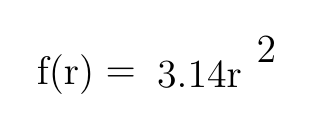
\begin{tikzpicture}
\node at (1.7,0) {{\Large 3.14r}};
\node at (2.55,0.32) {{\Large 2}};
\node at (0,0) {{\Large f(r)}};
\node at (0.7,0) {{\Large =}};
\end{tikzpicture}
\caption{Mathematical function for area of a circle}
\end{figure}

This function square the input value and multiply with 3.14.
Depending on the input value the output varies.

\begin{figure}[h!]
\centering
\begin{tikzpicture}
\draw [thick, ->] (0,1) -- (2,1);
\node at (.5,1.2) {r};
\draw [thick] (2,0) rectangle (7,2);
\node at (4.5,1) {3.14r};
\node at (5.1,1.2) {2};
\node at (4.5,2.3) {f(r)};
\draw [thick, ->] (7,1) -- (9,1);
\node at (8.5,1.2) {y};
\end{tikzpicture}
\caption{Blackbox representation of a function}
\end{figure}

As you can see in the above diagram, \texttt{r} is the input
and \texttt{y} is the output.  A function in Go can take input
arguments and perform actions and return values.  A simple
implementation of this function in Go looks like this.

\begin{lstlisting}[numbers=none]
func Area(r float64) float64 {
    return 3.14 * r * r
}
\end{lstlisting}

The function declaration starts with \texttt{func} keyword.  In the
above example, \texttt{Area} is the function name which can be later
used to call the function.  The arguments that can be received by this
function is given within brackets.  The line where function definition
started should end with an opening curly bracket.  The statements can
be written in the next line on wards until the closing curly bracket.

Here is a complete example with usage of the Area function.

\begin{lstlisting}[caption=Function usage]
package main

import "fmt"

// Area return the area of a circle for the given radius
func Area(r float64) float64 {
    return 3.14 * r * r
}

func main() {
    area := Area(5.0)
    fmt.Println(area)
}
\end{lstlisting}

In the above example, the \texttt{Area} function is called in line
number 11 with an argument of \texttt{5.0}.  We are using the short
variable declaration.  The type of the variable \texttt{area} will be
\texttt{float64} as the \texttt{Area} function returns with that type.

\subsection{Operators}

Programming languages use operators\index{operators} to simplify the
usage.  Operators behave more or less like functions.  More
specifically, operators combine operands to form expressions.  We have
already seen few operators
like \texttt{:=}, \texttt{=}, \texttt{+=}, \texttt{++}, \texttt{*},
\texttt{>} and \texttt{<}.

The \texttt{:=}, \texttt{=}, \texttt{+=} are assignment operators.
The \texttt{*} is the multiplication operator.  The \texttt{>}
and \texttt{<} are comparison operators.

Sometimes logical conditions should be checked to proceed with certain
steps.  Logical operators does these kind kind of checking.  Let's
say you want to check whether a particular value is divisible by 3
and 5.  You can do it like this.

\begin{lstlisting}[numbers=none]
if i%3 == 0 {
    if i%5 == 0 {
        // statements goes here
    }
}
\end{lstlisting}

The same thing can be achieved using conditional AND logical operator
(\texttt{\&\&}) like this.

\begin{lstlisting}[numbers=none]
if i%3 == 0 && i%5 == 0 {
    // statements goes here
}
\end{lstlisting}

Apart from the conditional AND, there are conditional OR (\texttt{||})
and NOT (\texttt{!}) logical operators.  We will see more about
operators in the next chapter.


\subsection{Slices}

Slice\index{slice} is a sequence of values of the same type.  In
computer science terminology, it's a homogeneous aggregate data type.
So, a slice can contain elements of only one type of data.  However,
it can hold a varying number of elements.  It can expand and shrink
the number of values.  \texttt{[]T} is a slice with elements of type
T.

The number of values in the slice is called the length of that slice.
The slice type \texttt{[]T} is a slice of type \texttt{T}.  Here is an
example slice of color names:

\begin{lstlisting}[numbers=none]
colors := []string{"Red", "Green", "Blue"}
\end{lstlisting}

In the above example, the length of slice is \texttt{3} and the slice
values are string data.  The \texttt{len} function gives the length of
slice.  See this complete example:

\begin{lstlisting}[caption=Printing slice values]
package main

import "fmt"

func main() {
    colors := []string{"Red", "Green", "Blue"}
    fmt.Println("Len:", len(colors))
    for i, v := range colors {
        fmt.Println(i, v)
    }
}
\end{lstlisting}

If you save the above program in a file named \texttt{colors.go} and
run it, you will get output like this:

\begin{lstlisting}[numbers=none]
$ go run colors.go
Len: 3
0 Red
1 Green
2 Blue
\end{lstlisting}

The \texttt{range}\index{range} clause loop over through elements in a
variety of data structures including slice and map.  Range gives index
and the value.  In the above example, the index is assigned
to \texttt{i} and value to \texttt{v} variables.  As you can see
above, each iteration change the value of \texttt{i} \& \texttt{v}.

If you are not interested in the index but just the value of string,
you can use blank identifier (variable).  In Go, underscore is
considered as blank identifier which you need not to define and you can
assign anything to it.  See the example written below to print each
string ignoring the index.

\begin{lstlisting}[caption=Range loop with index ignored]
package main

import "fmt"

func main() {
    colors := []string{"Red", "Green", "Blue"}
    fmt.Println("Len:", len(colors))
    for _, v := range colors {
        fmt.Println(v)
    }
}
\end{lstlisting}

If you just want to get the index without value, you can use just use
one variable to the left of range clause as give below.

\begin{lstlisting}[caption=Range loop without index]
package main

import "fmt"

func main() {
    colors := []string{"Red", "Green", "Blue"}
    fmt.Println("Len:", len(colors))
    for i := range colors {
        fmt.Println(i, colors[i])
    }
}
\end{lstlisting}

In the above example, we are accessing the value using the index
syntax: \texttt{colors[i]}.

\subsection{Maps}

Map\index{map} is another commonly used complex data structure in Go.
Map is an implementation of hash table which is available in many very
high level languages.  The data organized like key value pairs.  A
typical map type looks like this:

\begin{lstlisting}[numbers=none]
map[KeyType]ValueType
\end{lstlisting}

A \texttt{KeyType} can be any type that is comparable using the
comparison operators.  The \texttt{ValueType} can be any data type
including another map.  It is possible add any numbers of key value
pairs to the map.

Here is a map definition with some values initialized.

\begin{lstlisting}[numbers=none]
var fruits = map[string]int{
      "Apple":  45,
      "Mango":  24,
      "Orange": 34,
  }
\end{lstlisting}

To access a value corresponding to a key, you can use this syntax:

\begin{lstlisting}[numbers=none]
mangoCount := fruits["Mango"]
\end{lstlisting}

If the key doesn't exist, a zero value will be returned. For example, in the
below example, value of \texttt{pineappleCount} is going be \texttt{0}.

\begin{lstlisting}[numbers=none]
pineappleCount := fruits["Pineapple"]
\end{lstlisting}

More about maps will be explained in the data structure chapter.

\section{Exercises}

\textbf{Exercise 1:} Print multiples of 5 for all even numbers below 10

\textbf{Solution:}

This exercise requires getting all even numbers numbers below 10.  As
we we have seen above, a \texttt{for} loop can be used to get all
numbers.  Then \texttt{if} condition can be used with \texttt{\%}
operator to check whether the number is even or not.  The \texttt{\%}
operator given the gives the remainder and we can check it is zero or
not for modulus 2.  If the number is even use the \texttt{*} operator
to multiply with 5.

Here is the program.

\begin{lstlisting}[numbers=none]
package main

import "fmt"

func main() {
    for i := 1; i < 10; i++ {
        if i%2 == 0 {
            fmt.Println(i * 5)
        }
    }
}
\end{lstlisting}

\textbf{Exercise 2:} Create a function to reverse a string

\textbf{Solution:}

\begin{lstlisting}[numbers=none]
package main

import "fmt"

func Reverse(s string) string {
    var r string
    for _, c := range s {
        r = string(c) + r
    }
    return r
}

func main() {
    hw := "Hello, World!"
    rhw := Reverse(hw)
    fmt.Println(rhw)
}
\end{lstlisting}

\textbf{Exercise 3:} Find sum of all numbers below 50 completely divisible
by 2 or 3 (i.e., remainder 0).

Hint: The numbers completely divisible by 2 or 3 are 2, 3, 4, 6, 8, 9 ... 45,
46, 48.

\textbf{Solution:}

\begin{lstlisting}[numbers=none]
package main

import "fmt"

func main() {
    sum := 0
    for i := 1; i < 50; i++ {
        if i%2 == 0 {
            sum = sum + i
        } else {
            if i%3 == 0 {
                sum = sum + i
            }
        }
    }
    fmt.Println("Sum:", sum)
}
\end{lstlisting}

The logic can be simplified using a conditional OR operator.

\begin{lstlisting}[numbers=none]
package main

import "fmt"

func main() {
    sum := 0
    for i := 1; i < 50; i++ {
        if i%2 == 0 || i%3 == 0 {
            sum = sum + i
        }
    }
    fmt.Println("Sum:", sum)
}
\end{lstlisting}

\subsection{Additional Exercises}

Answers to these additional exercises are given in the Appendix A.

\textbf{Problem 1:} Write a function to check whether the first letter in a
given string is capital letters in English (A,B,C,D etc).

Hint: The signature of the function definition could be like this:
\texttt{func StartsCapital(s string) bool}.  If the function returns
\texttt{true}, the string passed starts with a capital letter.

\textbf{Problem 2:} Write a function to generate Fibonacci numbers below a
given value.

Hint: Suggested function signature: \texttt{func Fib(n int)}.  This
function can print the values.

\section*{Summary}

We started with a hello world program and briefly explained it.  Then
this chapter introduced few basic topics in Go programming language.
We have covered Data Types, Variables, Comments, For Loop, Range
Clause, If, Function, Operators, Slices, and Maps.  The next chapters
will explain the fundamental concepts in more detail.
